\documentclass[a4paper,10pt]{scrartcl}
\RequirePackage[hyperindex]{hyperref}
\usepackage{amssymb}
\begin{document}
\title{\texttt{cplint} on SWISH Manual}
\maketitle

%\section{Table of Contents}
%
%\begin{itemize}
%	\item \hyperref[syn]{Syntax} 
%	\item Inference \ref{inf}
%	\item Learning \ref{learning}
%\end{itemize}

\section{Syntax}
\label{syn}
\texttt{cplint} permits the definition of discrete probability distributions and continuous probaility
densities.
\subsection{Discrete Probability Distributions}
\label{discrete}
LPAD and CP-logic programs consist of a set of annotated disjunctive clauses.
Disjunction in the head is represented with a semicolon and atoms in the head are separated from probabilities by a colon. For the rest, the usual syntax of Prolog is used.
A general CP-logic clause has the form
\begin{verbatim}
h1:p1 ; ... ; hn:pn :- Body.
\end{verbatim}
where \verb|Body| is a conjunction of goals as in Prolog.
 No parentheses are necessary. The \texttt{pi} are numeric expressions. It is up to the user to ensure that the numeric expressions are legal, i.e. that they sum up to less than one.

If the clause has an empty body, it can be represented like this
\begin{verbatim}
h1:p1 ; ... ; hn:pn.
\end{verbatim}
If the clause has a single head with probability 1, the annotation can be omitted and the clause takes the form of a normal prolog clause, i.e. 
\begin{verbatim}
h1 :- Body.
\end{verbatim}
stands for 
\begin{verbatim}
h1:1 :- Body.
\end{verbatim}
The coin example of  \cite{VenVer04-ICLP04-IC} is represented as (file \href{http://cplint.eu/example/inference/coin.pl}{\texttt{coin.pl}})
\begin{verbatim}
heads(Coin):1/2 ; tails(Coin):1/2 :- 
  toss(Coin),\+biased(Coin).

heads(Coin):0.6 ; tails(Coin):0.4 :- 
  toss(Coin),biased(Coin).

fair(Coin):0.9 ; biased(Coin):0.1.

toss(coin).
\end{verbatim}
The first clause states that if we toss a coin that is not biased it has equal probability of landing heads and tails. The second states that if the coin is biased it has a slightly higher probability of landing heads. The third states that the coin is fair with probability 0.9 and biased with probability 0.1 and the last clause states that we toss a coin with certainty.

Moreover, the bodies of rules may contain built-in predicates, predicates
from the libraries \verb|lists|, \verb|apply| and \verb|clpr/nf_r|
plus the predicate
\begin{verbatim}
average/2
\end{verbatim}
that, given a list of numbers, computes its arithmetic mean.

The body of rules may also contain the predicate \verb|prob/2| that computes the
probability of an atom, thus allowing nested probability computations.
For example (\href{http://cplint.eu/example/inference/meta.pl}{\texttt{meta.pl}})
\begin{verbatim}
a:0.2:-
  prob(b,P),
  P>0.2.
\end{verbatim}
is a valid rule.

Moreover, the probabilistic annotations can be variables, as in 
(\href{http://cplint.eu/example/inference/flexprob.pl}{\texttt{flexprob.pl}}))
\begin{verbatim}
red(Prob):Prob.

draw_red(R, G):-
  Prob is R/(R + G),
  red(Prob).
\end{verbatim}
Variables in probabilistic annotations must be ground when resolution reaches the end of the body, 
otherwise an exception is raised.

Alternative ways of specifying probability distribution include
\begin{verbatim}
A:discrete(Var,D):-Body.
\end{verbatim}
or
\begin{verbatim}
A:finite(Var,D):-Body.
\end{verbatim}
where \verb|A| is an atom containg variable \verb|Var| and \verb|D|
is a list of couples \verb|Value:Prob| assigning probability \verb|Prob|
to \verb|Value|. 
Moreover, you can use
\begin{verbatim}
A:uniform(Var,D):-Body.
\end{verbatim}
where \verb|A| is an atom containg variable \verb|Var| and \verb|D|
is a list of values each taking the same probability (1 over the length
of \verb|D|).
\subsubsection{ProbLog Syntax}
You can also use ProbLog \cite{DBLP:conf/ijcai/RaedtKT07} syntax, so a general clause takes the form
\begin{verbatim}
p1::h1 ; ... ; pn::hn :- Body
\end{verbatim}
where the \texttt{pi} are numeric expressions. 

\subsubsection{PRISM Syntax}
You can also use PRISM \cite{DBLP:conf/ijcai/SatoK97} syntax, so a program is composed of
a set of regular Prolog rules whose body may contain calls to the \verb|msw/2| predicate (multi-ary 
switch). A call \verb|msw(term,value)| means that a random variable associated to \verb|term|
assumes value \verb|value|. The admissible values  for a discrete random variable are 
specified using facts for the \verb|values/2| predicate of the form
\begin{verbatim}
values(T,L).
\end{verbatim}
where \verb|T| is a term (possibly containing variables) and \verb|L| is a list of values.
The distribution over values is specified using directives for \verb|set_sw/2| of the form
\begin{verbatim}
:- set_sw(T,LP).
\end{verbatim}
where \verb|T| is a term (possibly containing variables) and \verb|LP| is a list of
probability values.
Remember that in PRISM each call to \verb|msw/2| refers to a different random
variable, i.e., no memoing is performed, differently from the case of LPAD/CP-Logic/ProbLog.

For example, the coin example above in PRISM syntax becomes
(\href{http://cplint.eu/example/inference/coinmsw.pl}{\texttt{coinmsw.pl}})
\begin{verbatim}
values(throw(_),[heads,tails]).
:- set_sw(throw(fair),[0.5,0.5]).
:- set_sw(throw(biased),[0.6,0.4]).
values(fairness,[fair,biased]).
:- set_sw(fairness,[0.9,0.1]).
res(Coin,R):- toss(Coin),fairness(Coin,Fairness),msw(throw(Fairness),R).
fairness(_Coin,Fairness) :- msw(fairness,Fairness).
toss(coin).
\end{verbatim}
\subsection{Continuous Probability Densities}
\label{cont}

\verb|cplint| handles continuous random variables as well with its
sampling inference module.
To specify a probability density on an argument \verb|Var| of an atom
\verb|A| you can used rules of the form
\begin{verbatim}
A:Density:- Body
\end{verbatim}
where \verb|Density| is a special atom identifying a probability  density on variable \verb|Var| and \verb|Body| (optional) is a regular clause body.
Allowed \verb|Density| atoms are
\begin{itemize}
\item \verb|uniform(Var,L,U)|: \verb|Var| is uniformly distributed in $[L,U]$
\item \verb|gaussian(Var,Mean,Variance)|: \verb|Var| follows a Gaussian distribution with mean \verb|Mean| and variance \verb|Variance|. The distribution can be multivariate if \verb|Mean| 
is a list and \verb|Variance| a list of lists representing the mean vector and the covariance matrix. In this case the values of \verb|Var| are lists of real values with the same length as
that of \verb|Mean|
\item \verb|dirichlet(Var,Par)|: \verb|Var| is a list of real
numbers following a Dirichlet distribution with $\alpha$ parameters specified
by the list \verb|Par|
\item \verb|gamma(Var,Shape,Scale)|  \verb|Var| follows a gamma distribution 
with shape parameter \verb|Shape| and scale parameter \verb|Scale|.
\item \verb|beta(Var,Alpha,Beta)|  \verb|Var| follows a beta distribution 
with parameters \verb|Alpha| and \verb|Beta|.
\item \verb|poisson(Var,Lambda)|  \verb|Var| follows a Poisson distribution 
with parameter \verb|Lambda|.
\item \verb|binomial(Var,N,P)|  \verb|Var| follows a binomial distribution 
with parameters \verb|N| and \verb|P|.
\item \verb|geometric(Var,P)|  \verb|Var| follows a geometric distribution 
with parameter \verb|P|.
\end{itemize}
For example
\begin{verbatim}
g(X): gaussian(X,0, 1).
\end{verbatim}
states that argument \verb|X| of \verb|g(X)| follows a Gaussian 
distribution with mean 0 and variance 1, while
\begin{verbatim}
g(X): gaussian(X,[0,0], [[1,0],[0,1]]).
\end{verbatim}
states that argument \verb|X| of \verb|g(X)| follows a Gaussian 
multivariate distribution with mean vector $[0,0]$ and covariance matrix
$$\left[\begin{array}{rr}
1&0\\
0&1
\end{array}\right]$$.



For example, \href{http://cplint.eu/example/inference/gaussian_mixture.pl}{\texttt{gaussian\_mixture.pl}} defines a mixture of two Gaussians:
\begin{verbatim}
heads:0.6;tails:0.4.
g(X): gaussian(X,0, 1).
h(X): gaussian(X,5, 2).
mix(X) :- heads, g(X).
mix(X) :- tails, h(X).
\end{verbatim}
The argument \verb|X| of
\verb|mix(X)| follows a distribution that is a mixture of two Gaussian,
one with mean 0 and variance 1 with probability 0.6 and one with 
mean 5 and variance 2 with probability 0.4.

The parameters of the distribution atoms can be taken from the probabilistic
atom, the example \href{http://cplint.eu/example/inference/gauss_mean_est.pl}{\texttt{gauss\_mean\_est.pl}}
\begin{verbatim}
val(I,X) :-
  mean(M),
  val(I,M,X).
mean(M): gaussian(M,1.0, 5.0).
val(_,M,X): gaussian(X,M, 2.0).
\end{verbatim}
states that for an index \verb|I| the continuous variable \verb|X| is 
sampled from a Gaussian whose variance is 2 and whose mean is sampled from a Gaussian with mean 1 and
variance 5.

Any operation is allowed on continuous random variables. The example below
(\href{http://cplint.eu/example/inference/kalman_filter.pl}{\texttt{kalman\_filter.pl}}) encodes a Kalman filter:
\begin{verbatim}
kf(N,O, T) :-
  init(S),
  kf_part(0, N, S,O,T).
kf_part(I, N, S,[V|RO], T) :-
  I < N,
  NextI is I+1,
  trans(S,I,NextS),
  emit(NextS,I,V),
  kf_part(NextI, N, NextS,RO, T).
kf_part(N, N, S, [],S).
trans(S,I,NextS) :-
  {NextS =:= E + S},
  trans_err(I,E).
emit(NextS,I,V) :-
  {NextS =:= V+X},
  obs_err(I,X).
init(S):gaussian(S,0,1).
trans_err(_,E):gaussian(E,0,2).
obs_err(_,E):gaussian(E,0,1).
\end{verbatim}
Continuous random variables are involved
in arithmetic expressions (in \verb|trans/3| and \verb|emit/3|). It
is often convenient, as in this case, to use CLP(R) constraints (by
including the directive \verb|:- use_module(library(clpr)).|) as 
in this way the expressions can be used in multiple directions and 
the same clauses can be used both to sample and to evaluate the weight the sample on the basis
of evidence,
otherwise different clauses have to be written.
In case random variables are not sufficiently instantiated to 
exploit expressions for inferring the values of other variables, 
inference will return an error.

\subsubsection{Distributional Clauses Syntax}
\label{dc}
You can also use the syntax of Distributional Clauses (DC) \cite{Nitti2016}.
Continuous random variables are represented in this case by term whose distribution can be specified with density atoms as in
\begin{verbatim}
T~Density' := Body.
\end{verbatim}
Here \verb|:=| replaces the implication symbol, \verb|T| is a term and \verb|Density'| is one of the density atoms above without the \verb|Var| argument, because \verb|T|
itself represents a random variables. In the body of clauses you can use the infix operator \verb|~=| to equate a term representing a random variable with a logical variable or
a constant as in \verb|T ~= X|. Internally \verb|cplint| transforms the terms representing random variables into atoms with an extra argument for holding the variable.
DC can be used to represent also discrete distributions using
\begin{verbatim}
T~uniform(L) := Body.
T~finite(D) := Body.
\end{verbatim} 
where \verb|L| is a list of values and \verb|D| is a list of couples \verb|P:V| with \verb|P| a probability and \verb|V| a value.
If \verb|Body| is empty, as in regular Prolog, the implication symbol \verb|:=| can be omitted.

The Indian GPA problem from \url{http://www.robots.ox.ac.uk/~fwood/anglican/examples/viewer/?worksheet=indian-gpa}in distributional clauses syntax  (\url{https://github.com/davidenitti/DC/blob/master/examples/indian-gpa.pl})
takes the form (\href{http://cplint.eu/example/inference/indian_gpadc.pl}{\texttt{indian\_gpadc.pl}}):
\begin{verbatim}
is_density_A:0.95;is_discrete_A:0.05.
% the probability distribution of GPA scores for American students is
% continuous with probability 0.95 and discrete with probability 0.05

agpa(A): beta(A,8,2) :- is_density_A.
% the GPA of American students follows a beta distribution if the
% distribution is continuous

american_gpa(G) : finite(G,[4.0:0.85,0.0:0.15]) :- is_discrete_A.
% the GPA of American students is 4.0 with probability 0.85 and 0.0
% with 
% probability 0.15 if the
% distribution is discrete
american_gpa(A):- agpa(A0), A is A0*4.0.
% the GPA of American students is obtained by rescaling the value of
% agpa
% to the (0.0,4.0) interval
is_density_I : 0.99; is_discrete_I:0.01.
% the probability distribution of GPA scores for Indian students is
% continuous with probability 0.99 and discrete with probability 
% 0.01
igpa(I): beta(I,5,5) :- is_density_I.
% the GPA of Indian students follows a beta distribution if the
% distribution is continuous
indian_gpa(I): finite(I,[0.0:0.1,10.0:0.9]):-  is_discrete_I.
% the GPA of Indian students is 10.0 with probability 0.9 and 0.0
% with
% probability 0.1 if the
% distribution is discrete
indian_gpa(I) :- igpa(I0), I is I0*10.0.
% the GPA of Indian students is obtained by rescaling the value 
% of igpa
% to the (0.0,4.0) interval
nation(N) : finite(N,[a:0.25,i:0.75]).
% the nation is America with probability 0.25 and India with 
% probability 0.75
student_gpa(G):- nation(a),american_gpa(G).
% the GPA of the student is given by american_gpa if the nation is 
% America
student_gpa(G) :- nation(i),indian_gpa(G).
% the GPA of the student is given by indian_gpa if the nation 
%is India
\end{verbatim}
See 

\section{Semantics}
\label{semantics}

The semantics of LPADs for the case of programs without functions symbols can be given
as follows. An LPAD defines a probability distribution over normal logic programs called
\emph{worlds}. A world is obtained from an LPAD by first grounding it, by 
selecting a single head atom for each ground clause and by including in the world
the clause with the selected head atom and the body.
The probability of a world is the product of the probabilities associated to the 
heads selected.
The probability of a ground atom (the query) is given by the sum of the probabilities
of the worlds where the query is true.

If the LPAD contains function symbols, the definition is more complex, see
\cite{DBLP:journals/ai/Poole97,DBLP:journals/jair/SatoK01,Rig15-PLP-IW}.

For the semantics of programs with continuous random variables, see \cite{TLP:8688161}
that defines the probability
space for $N$ continuous random variables by considering the Borel $\sigma$-algebra
over $\mathbb{R}^N$
and defines a Lebesgue measure on this set as the probability measure.
The probability space is lifted to cover the entire program using the least model semantics of constraint logic programs. Alternatively,
\cite{Nitti2016} defines the semantics of distributional clauses by resorting to
a stochastic $Tp$ operator.
\verb|cplint| allows more freedom than distributional clauses in the use of continuous random variables
in expressions, for example
\href{http://cplint.eu/e/kalman_filter.pl}{\texttt{kalman\_filter.pl}} would not be allowed by distributional clauses.

\section{Inference}
\label{inf}

TRILL systems can answer many different queries. To do so, it exploits an algorithm called \emph{tableau} algorithm, which is able to collect explanations. In the following you can find an example that shows how the tableau works. In section~\ref{sec:trillq} we will see how queries can be asked with TRILL systems.

Consider a simple knowledge base inspired by the film ``The Godfather'' containing the following axioms:
\begin{align}
&tom : Cat\\
&(donVito, tom) : hasPet\\
&Cat \sqsubseteq Pet\\
&\exists hasAnimal.Pet \sqsubseteq NatureLover\\
&NatureLover \sqsubseteq GoodPerson\\
&hasPet \sqsubseteq hasAnimal
\end{align}

The axioms are telling what is known about the domain: (1) Tom is an individual of the domain, and he is a Cat; (2) donVito (Vito Corleone) has tom as his pet; (3) all cats are also pets; (4) everyone having at least one animal which is a pet is a nature lover; (5) nature lovers are good people; and (6) if one has a pet, she/he also has an animal.

This KB can be defined by the following TRILL syntax axioms:
\begin{verbatim}
classAssertion(cat, tom).
propertyAssertion(hasPet, donVito, tom).
subClassOf(cat, pet).
subClassOf(someValuesFrom(hasAnimal, pet), natureLover).
subClassOf(natureLover,goodPerson).
subPropertyOf(hasPet,hasAnimal).
\end{verbatim}

The first two axioms are assertional axioms (hence they constitute the ABox), the other four axioms define the TBox. Axiom 1 is called class assertion, 2 is called property assertion, 3,4,5 are called class subsumption axioms, and axiom 6 is called property subsumption axiom.

To check, for example, whether don Vito Corleone is a good person, the tableau algorithm builds a graph, called the \emph{tableau}. The initial tableau contains information from the ABox plus the negation of the query, as depicted in Figure\ref{fig:tab1}. This last axiom is added since the underlying proof mechanism uses refutation. In logic, working by refutation means assuming the opposite of the query one wants to prove. Then, if this assumption leads to a contradiction, this means that the axioms of the ontology allows to prove that the query is true, and thus that its opposite is false. In practice, working by refutation means that the graph must assume that the posed query be false, the tableau algorithm expands all the known axioms (including the negation of the query) and looks for contradictions present in the final graph. The presence of a contradiction in a node proves that the query is true because the graph depicts at least one way to contradict the negation of that query, and thus it depicts at least one way to prove that the opposite of the query contradicts what is defined by the ontology. 

\begin{figure}
	\centering
	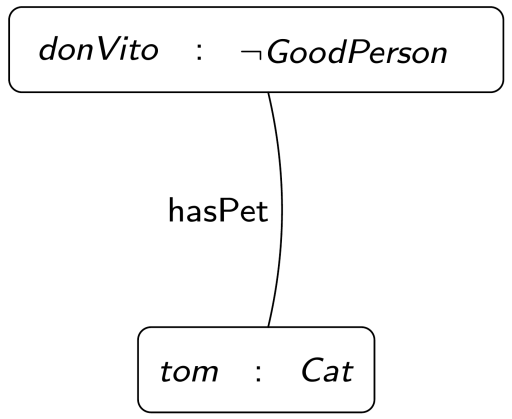
\includegraphics[width=0.5\linewidth]{img/tab1}
	\caption{Initial tableau}
	\label{fig:tab1}
\end{figure}

This means that if the opposite of the query is (artificially) added to the knowledge base as a new axiom, this ontology will contain at least two pieces of information one contradicting the other.

The tableau has one node for each individual: tom is labelled as cat, $donVito$ is labelled as not a good person (the negation of the query), and the edge between them is labelled as $hasPet$ because the individuals are connected by this property (Figure~\ref{fig:tab1}).

At this point, the graph of Figure~\ref{fig:tab1} is expanded using the axioms of the ontology to check the truth of the query and to build the justifications. Therefore, the tableau algorithm takes e.g. the axiom 3, ``cats are pets'', and adds to the node for tom also the label $pet$ since he is a cat. This new information is true and its justification is given directly by the set of axioms {1,3}: axiom 3 because since $tom$ is a $cat$ (axiom 1) he is also a $pet$. The same operation can be done for the edge (relationship) between tom and $donVito$, which can be labelled also as $hasAnimal$ because of axioms~2 and~6.

At this point, the calculus can deduce that $donVito$ belongs to the class \linebreak $\exists hasAnimal.Pet$ because $donVito$ is connected with $tom$, which is a $pet$ (axioms {1,3}), via property $hasAnimal$ (axioms {2,6}). Therefore, $donVito$’s node is labelled also as $\exists hasAnimal.Pet$ with a justification given by the union of the axioms associated with the used axioms, therefore its justification is given by the set of the involved axioms {1,2,3,6}. Then, the tableau graph is further expanded by adding the class $NatureLover$ to $donVito$’s node using axiom 4 and finally, by adding also the class $GoodPerson$ using label $NatureLover$ (axioms {1,2,3,4,6}) and axiom 5, creating as justification the set of axioms {1,2,3,4,5,6}.

The final graph is shown in Figure~\ref{fig:tab2}.
\begin{figure}
	\centering
	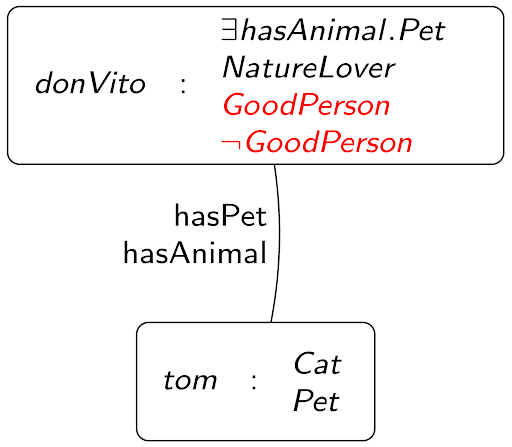
\includegraphics[width=0.5\linewidth]{img/tab2}
	\caption{Initial tableau}
	\label{fig:tab2}
\end{figure}
The expanded graph contains now a contradiction, i.e., $donVito$ is labelled as $GoodPerson$ and as not a $GoodPerson$ (i.e., $\neg GoodPerson$), therefore, by refutation, the query ``Is don Vito Corleone a good person?'' is true, with justification given by the axioms {1,2,3,4,5,6}, that are the axioms of the KB necessary to deduce this information.

From this example, it would be clear why the use of probabilistic information is useful. Indeed, don Vito Corleone is hardly classifiable as a good person. This is because not all people who are nature lovers are also good, and therefore, one could say that axiom 5 is true with probability 0.4. It would also be arguable that everyone who has animals is also a nature lover, making probabilistic also this axiom. For a formal description of how the probability of the query is computed see the Appendix~\ref{app:inf}.

\subsection{Possible Queries}
\label{queries}

TRILL can compute the probability or find an explanation of the following queries:
\begin{itemize}
  \item Concept membership queries.
  \item Property assertion queries.
  \item Subsumption queries.
  \item Unsatifiability of a concept.
  \item Inconsistency of the knowledge base.
\end{itemize}
All the input arguments must be atoms or ground terms.
Note that it is necessary to specify which algorithm, TRILL, TRILL$^P$ or TORNADO, has to be loaded for performing inference. This is done by using at the beginning of the input file the directive
\begin{verbatim}
:- trill.
\end{verbatim}
for loading TRILL,
\begin{verbatim}
:- trillp.
\end{verbatim}
for TRILL$^P$ or
\begin{verbatim}
:- tornado.
\end{verbatim}
for TORNADO.

\subsubsection{Probabilistic Queries}
TRILL can be queried for computing the probability of queries. A resulting 0 probaility means that the query is false w.r.t. the knowledge base, while a probability value 1 that the query is certainly true.

The probability of an individual to belong to a concept can be asked using TRILL with the predicate
\begin{verbatim}
prob_instanceOf(+Concept:term,+Individual:atom,-Prob:double)
\end{verbatim}
as in (\href{http://trill.lamping.unife.it/example/trill/peoplePets.pl}{\texttt{peoplePets.pl}})
\begin{verbatim}
?- prob_instanceOf(cat,'Tom',Prob).
\end{verbatim}

The probability of two individuals to be related by a role can be computed with
\begin{verbatim}
prob_property_value(+Prop:atom,+Individual1:atom,
                    +Individual2:atom,-Prob:double)
\end{verbatim}
as in (\href{http://trill.lamping.unife.it/example/trill/peoplePets.pl}{\texttt{peoplePets.pl}})
\begin{verbatim}
?- prob_property_value(has_animal,'Kevin','Tom',Prob).
\end{verbatim}

If you want to know the probability with which a class is a subclass of another you have to use
\begin{verbatim}
prob_sub_class(+Concept:term,+SupConcept:term,-Prob:double)
\end{verbatim}
as in (\href{http://trill.lamping.unife.it/example/trill/peoplePets.pl}{\texttt{peoplePets.pl}})
\begin{verbatim}
?- prob_sub_class(cat,pet,Prob).
\end{verbatim}

The probability of the unsatisfiability of a concept can be asked with the predicate
\begin{verbatim}
prob_unsat(+Concept:term,-Prob:double)
\end{verbatim}
as in (\href{http://trill.lamping.unife.it/example/trill/peoplePets.pl}{\texttt{peoplePets.pl}})
\begin{verbatim}
?- prob_unsat(intersectionOf([cat,complementOf(pet)]),P).
\end{verbatim}
This query for example corresponds with a subsumption query, which is represented as the intersection of the subclass and the complement of the superclass.

Finally, you can ask the probability of the inconsistency of the knowledge base with
\begin{verbatim}
prob_inconsistent_theory(-Prob:double)
\end{verbatim}


\subsubsection{Non Probabilistic Queries}
In TRILL you can also ask whether a query is true or false w.r.t. the knowledge base and in case of a succesful query an explanation can be returned as well. 
Query predicates in this case differs in the number of arguments, in the second case, when we want also an explanation, an extra argument is added to unify with the list of axioms
build to explain the query.

The query if an individual belongs to a concept can be used the predicates
\begin{verbatim}
instanceOf(+Concept:term,+Individual:atom)
instanceOf(+Concept:term,+Individual:atom,-Expl:list)
\end{verbatim}
as in (\href{http://trill.lamping.unife.it/example/trill/peoplePets.pl}{\texttt{peoplePets.pl}})
\begin{verbatim}
?- instanceOf(pet,'Tom').
?- instanceOf(pet,'Tom',Expl).
\end{verbatim}
In the first query the result is \verb|true| because Tom belongs to cat, in the second case TRILL returns the explanation 
\begin{verbatim}
[classAssertion(cat,'Tom'), subClassOf(cat,pet)]
\end{verbatim}


Similarly, to ask whether two individuals are related by a role you have to use the queries
\begin{verbatim}
property_value(+Prop:atom,+Individual1:atom,+Individual2:atom)
property_value(+Prop:atom,+Individual1:atom,
               +Individual2:atom,-Expl:list)
\end{verbatim}
as in (\href{http://trill.lamping.unife.it/example/trill/peoplePets.pl}{\texttt{peoplePets.pl}})
\begin{verbatim}
?- property_value(has_animal,'Kevin','Tom').
?- property_value(has_animal,'Kevin','Tom',Expl).
\end{verbatim}

If you want to know if a class is a subclass of another you have to use
\begin{verbatim}
sub_class(+Concept:term,+SupConcept:term)
sub_class(+Concept:term,+SupConcept:term,-Expl:list)
\end{verbatim}
as in (\href{http://trill.lamping.unife.it/example/trill/peoplePets.pl}{\texttt{peoplePets.pl}})
\begin{verbatim}
?- sub_class(cat,pet).
?- sub_class(cat,pet,Expl).
\end{verbatim}

The unsatisfiability of a concept can be asked with the predicate
\begin{verbatim}
unsat(+Concept:term)
unsat(+Concept:term,-Expl:list)
\end{verbatim}
as in (\href{http://trill.lamping.unife.it/example/trill/peoplePets.pl}{\texttt{peoplePets.pl}})
\begin{verbatim}
?- unsat(intersectionOf([cat,complementOf(pet)])).
?- unsat(intersectionOf([cat,complementOf(pet)]),Expl).
\end{verbatim}
In this case, the returned explanation is the same obtained by querying if cat is subclass of pet with the \verb|sub_class/3| predicate, i.e., \verb|[subClassOf(cat,pet)]|

Finally, you can ask about the inconsistency of the knowledge base with
\begin{verbatim}
inconsistent_theory
inconsistent_theory(-Expl:list)
\end{verbatim}

The predicate above returns explanations one at a time. To collect all the explanations with a single goal you can use the predicates:
\begin{verbatim}
all_instanceOf(+Concept:term,+Individual:atom,-Expl:list)
all_property_value(+Prop:atom,+Individual1:atom,
                        +Individual2:atom,-Expl:list)
all_sub_class(+Concept:term,+SupConcept:term,-Expl:list)
all_unsat(+Concept:term,-Expl:list)
all_inconsistent_theory(-Expl:list)
\end{verbatim}

\subsection{Query Options}
The behaviour of the queries can be fine tuned using the \emph{query options}. To use them you need to use the predicates:
\begin{verbatim}
instanceOf(+Concept:term,+Individual:atom,-Expl:list,-QueryOptions:list)
property_value(+Prop:atom,+Individual1:atom,
                        +Individual2:atom,-Expl:list,-QueryOptions:list)
sub_class(+Concept:term,+SupConcept:term,-Expl:list,-QueryOptions:list)
unsat(+Concept:term,-Expl:list,-QueryOptions:list)
inconsistent_theory(-Expl:list,-QueryOptions:list)
\end{verbatim}

Options can be:
\begin{itemize}
	\item \verb|assert_abox(Boolean)| if Boolean is set to true the list of ABoxes is asserted with the predicate \verb|final_abox/1|;
	\item \verb|return_prob(Prob)| if present the probability of the query is computed and unified with \verb|Prob|;
%	\item \verb|return_single_prob(Boolean)| must be used with \verb|return_prob(Prob)|. It forces TRILL to return the probability of each single explanation;
	\item \verb|max_expl(Value)| to limit the maximum number of explanations to find. \verb|Value| must be an integer. The predicate will return a list containing at most \verb|Value| different explanations;
	\item \verb|time_limit(Value)| to limit the time for the inference. The predicate will return the explanations found in the time allowed. \verb|Value| is the number of seconds allowed for the search of explanations .
\end{itemize}

For example, if you want to find the probability of the query $Q=kevin:PetOwner$ computed on at most 2 explanations allowing at most 1 second for the explanations search you can use the goal
\begin{verbatim}
instanceOf('natureLover','Kevin',Expl,
           [time_limit(1),return_prob(Prob),max_expl(2)]).
\end{verbatim}

\subsection{TRILL Useful Predicates}
There are other predicates defined in TRILL which helps manage and load the KB.
\begin{verbatim}
add_kb_prefix(++ShortPref:string,++LongPref:string)
add_kb_prefixes(++Prefixes:list)
\end{verbatim}
They register the alias for prefixes. The firs registers \verb|ShortPref| for the prefix \verb|LongPref|, while the second register all the alias prefixes contained in Prefixes. The input list must contain pairs alias=prefix, i.e., \verb|[('foo'='http://example.foo#')]|. In both cases, the empty string \verb|''| can be defined as alias. The predicates
\begin{verbatim}
remove_kb_prefix(++ShortPref:string,++LongPref:string)
remove_kb_prefix(++Name:string)
\end{verbatim}
remove from the registered aliases the one given in input. In particular, \verb|remove_kb_prefix/1| takes as input a string that can be an alias or a prefix and removes the pair containing the string from the registered aliases.

\begin{verbatim}
add_axiom(++Axiom:axiom)
add_axioms(++Axioms:list)
\end{verbatim}
These predicates add (all) the given axiom to the knowledge base. While, to remove axioms can be similarly used the predicates
\begin{verbatim}
remove_axiom(++Axiom:axiom)
remove_axioms(++Axioms:list)
\end{verbatim}
All the axioms must be defined following the TRILL syntax.

Finally, we can interrogate TRILL to return the loaded axioms with
\begin{verbatim}
axiom(?Axiom:axiom)
\end{verbatim}
This predicate searches in the loaded knowledge base axioms that unify with Axiom.


\subsection{Graphing the Results}
\label{graphing}

In \texttt{cplint} on SWISH you can draw graphs
for visualizing the results either with \href{http://www.c3js.org/}{C3.js} or with \href{https://www.r-project.org/}{R}. Similar predicates are available for the two methods.
 There are two types
of graphs: those that represent individual probability values with a bar chart and those that
visualize the results of sampling arguments.

\subsubsection{Using C3.js}
You can draw the probability of a query being true and
being false as a bar chart using the predicates
\begin{verbatim}
bar1(+Probability:float,-Chart:dict) is det
bar(+Probability:float,-Chart:dict) is det
bar(+Successes:int,+Failures:int,-Chart:dict) is det
argbar(+Values:list,-Chart:dict) is det
\end{verbatim}
They return  a dict for rendering with C3.js as a bar chart:
the first  returns bar chart with
a single bar for the probability,  the second a chart with
bar for the probability and a bar for one minus the probability,
the third a  chart with
a bar for the number of successes and a bar for the number of failures, and
the fourth a  chart with
a for bar each value, where \verb|Values| is a list of couples \verb|V-N| where
  \verb|V| is the value and \verb|N| is the number of samples
  returning that value.
 
To render C3.js charts  you have to include
\begin{verbatim}
:- use_rendering(c3).
\end{verbatim}
before \verb|:- pita.| 

You can also use the  \verb|bar(-Chart:dict)| option of many predicates
as in
\begin{verbatim}
?- prob(heads(coin),biased(coin),P,[bar(Chart)]).
\end{verbatim}
\verb|P| will be instantiated with a
 chart with
a bar for the probability of \verb|heads(coin)| true and a bar for the probability of \verb|heads(coin)| false,
given that \verb|biased(coin)| is true.

Another example is
\begin{verbatim}
?- mc_prob(heads(coin),P,[bar(Chart)]).
\end{verbatim}
that returns a chart representation of the probability.
\begin{verbatim}
?- mc_sample(heads(coin),1000,P,[bar(Chart)]).
\end{verbatim}
returns in \verb|Chart| a diagram with one bar for the number of successes and
one bar for the number of failures.

The options of
\verb|mc_sample_arg/5|, \verb|mc_sample_arg_first/5|,   \verb|mc_mh_sample_arg/6|,  \verb|mc_rejection_sample_arg/6|, 
can be used for visualizing the results of sampling arguments.

An example is
\begin{verbatim}
?- mc_sample_arg(reach(s0,0,S),50,S,ValList,[bar(Chart)]).
\end{verbatim}
of \href{http://cplint.eu/example/inference/markov_chain.pl}{\texttt{markov\_chain.pl}}.

The same result can be achieved with
\begin{verbatim}
?- mc_sample_arg(reach(s0,0,S),50,S,ValList),argbar(ValList,Chart)
\end{verbatim}
Drawing a graph is particularly interesting when
sampling values for continuous arguments of goals.
In this case, you can use the samples to draw the
probability density function of the argument.
The predicate
\begin{verbatim}
histogram(+List:list,-Chart:dict,+Options:list) is det
\end{verbatim}
draws a histogram of the samples in \verb|List| that  must be a list of couples of the form \verb|[V]-W| or  \verb|V-W|
where \verb|V| is a sampled value and \verb|W| is its weight. This is the format of the list of samples returned by argument sampling predicates.

The predicate
\begin{verbatim}
density(+List:list,-Chart:dict,+Options:list) is det
\end{verbatim}
draws a line chart of the density of  the samples in \verb|List| that  must take the same form as for \verb|histogram/3|.

In  \verb|histogram/3| and  \verb|density/3| \verb|Options| is a list of options, the following are recognised: \begin{itemize}
\item \verb|min(+Min:float)|
the minimum value of domain, default value the minimum in \verb|List|
\item \verb|max(+Max:float)|
the maximum value of domain, default value the maximum in  \verb|List|
\item \verb|nbins(+NBins:int)|
  the number of bins for dividing the domain, default value 40
\end{itemize}
In this way you can specify the limits and the number of intervals of the $X$.


The predicate
\begin{verbatim}
densities(+PriorList:list,+PostList:list,-Chart:dict,
  +Options:list) is det
\end{verbatim}
draws a line chart of the density of two sets of samples, usually
 prior and post observations. The samples in \verb|PriorList| and \verb|PostList|
can be either couples \verb|[V]-W| or \verb|V-W| where \verb|V| is a value and \verb|W| its weight.
The same options as for \verb|histogram/3| and  \verb|density/3|  are recognized.

For example, the query
\begin{verbatim}
?-  mc_sample_arg(value(0,X),1000,X,L0,[]),
    histogram(L0,Chart,[]).
\end{verbatim}
from \href{http://cplint.eu/example/inference/gauss_mean_est.pl}{\texttt{gauss\_mean\_est.pl}},
takes 1000 samples of argument \verb|X| of \verb|value(0,X)| and draws the density of the samples using an histogram.

Instead
\begin{verbatim}
?- mc_sample_arg(value(0,Y),1000,Y,L0,[]),
   mc_lw_sample_arg(value(0,X),
    (value(1,9),value(2,8)),1000,X,L),
   densities(L0,L,Chart).
\end{verbatim}
from \href{http://cplint.eu/example/inference/gauss_mean_est.pl}{\texttt{gauss\_mean\_est.pl}}
takes 1000 samples of argument \verb|X| of \verb|value(0,X)| before and after observing
\verb|(value(1,9),value(2,8)| and draws the prior and posterior densities of the samples using a line chart.

Predicates \verb|histogram/3|,  \verb|density/3|  and  \verb|densities/4| each have a version with one 
argument less that is equivalent to the predicate called with an empty option list.

\subsubsection{Using R}
You have to load library \texttt{cplint\_r}  (a SWI-Prolog pack) with
\begin{verbatim}
:- use_module(library(cplint_r)).
\end{verbatim}
Then you can use predicates
\begin{verbatim}
bar_r/1
bar_r/2
argbar_r/1
\end{verbatim}
that work as their C3.js counterpart but do not return the graph as an argument as the graph is
printed with a different mechanism.

You also have
\begin{verbatim}
histogram_r(+List:list,+Options:list) is det
\end{verbatim}
that works as \texttt{histogram/3}.
\begin{verbatim}
density_r(+List:list) is det
\end{verbatim}
is like \texttt{density/3} with the number of bins  is determined
by R.
\begin{verbatim}
densities_r(+PriorList:list,+PostList:list) is det
\end{verbatim}
is like \texttt{densities/3} with the number of bins  is determined
by R.

See \href{http://cplint.eu/example/inference/gauss_mean_est_R.pl}{\texttt{gauss\_mean\_est\_R.pl}} for an example of use of these predicates.




ml\subsection{Parameters}
The inference modules have a number of parameters in order to control their behavior. They can be set with the directive
\begin{verbatim}
:- set_pita(<parameter>,<value>).
\end{verbatim}
or
\begin{verbatim}
:- set_mc(<parameter>,<value>).
\end{verbatim}
after initialization (\verb|:-pita.| or \verb|:-mc.|) but outside \verb|:-begin/end_lpad.|
The current value can be read with
\begin{verbatim}
?- setting_pita(<parameter>,Value).
\end{verbatim}
or
\begin{verbatim}
?- setting_mc(<parameter>,Value).
\end{verbatim}
from the top-level.
The available parameters common to both \verb|pita| and \verb|mcintyre| are:
\begin{itemize}
\item 
	 \verb|epsilon_parsing|: if (1 - the sum of the probabilities of all the head atoms) is larger than 
    \verb|epsilon_parsing|,
		then \texttt{pita} adds the null event to the head. Default value \texttt{0.00001}.
\item \verb|single_var|: determines how non ground clauses are treated: if \texttt{true}, a single random variable is assigned to the whole non ground clause, 
if \texttt{false}, a different random variable is assigned to every grounding of the clause. Default value \texttt{false}.
\end{itemize}
Moreover, \verb|pita| has the parameters
\begin{itemize}
\item \verb|depth_bound|: if \texttt{true}, the depth of the derivation of the goal is limited to the value of the \texttt{depth} parameter.  Default value \texttt{false}.
\item  \texttt{depth}: maximum depth of derivations when  \verb|depth_bound| is set to \texttt{true}. Default value \texttt{5}.
\item \verb|prism_memoization|: \verb|false|: original prism semantics, \verb|true|: semantics with memoization
\end{itemize}
If \verb|depth_bound| is set to \verb|true|, derivations are depth-bounded so you can query also programs
containing infinite loops, for example programs where queries have an infinite number of explanations. However the probability that is returned is guaranteed only to be a lower bound,
see for example \href{http://cplint.eu/e/markov_chaindb.pl}{\texttt{markov\_chaindb.pl}}

\verb|mcintyre| has the parameters
\begin{itemize}
\item \verb|min_error|: minimal width of the binomial proportion confidence interval for the probability of the query. When the confidence interval for the probability of the query is below \verb|min_error|, 
the computation stops.
 Default value \verb|0.01|.
\item 
\verb|k|:  the number of samples to take before checking whether the the binomial proportion confidence interval is below \verb|min_error|.
Default value \verb|1000|.
\verb|max_samples|: the maximum number of samples to take. This is used when the probability of the
query is very close to 0 or 1. In fact \verb|mcintyre| also checks for the validity of the
the binomial proportion confidence interval: if less than 5 failures or successes are sampled,
even if the width of the confidence interval is less than \verb|min_error|, the computation continues.
This would lead to non-termination in cases where the probability is 0 or 1. 
\verb|max_samples| ensures termination.
 Default value \verb|10e4|.
\item \verb|prism_memoization|: \verb|false|: original prism semantics, \verb|true|: semantics with memoization
\end{itemize}
The example \href{http://cplint.eu/e/markov_chain.pl}{\texttt{markov\_chain.pl}}
shows that \verb|mcintyre| can perform inference in presence of an infinite number of explanations for 
the goal. Differently from \verb|pita|, no depth bound is necessary, as the probability of selecting
the infinite computation branch is 0. However, also \verb|mcintyre| may not terminate if loops not
involving probabilistic predicates are present.

If you want to set the seed of the random number generator, you can use SWI-Prolog predicates \verb|setrand/1| and \verb|getrand/1|, see
\href{http://www.swi-prolog.org/pldoc/doc_for?object=setrand/1}{SWI-Prolog manual}.

\subsection{Tabling}
You can also use tabling in inference to speed up the computation and/or avoid loops, see
the \href{http://www.swi-prolog.org/pldoc/man?section=tabling}{SWI-Prolog manual}.

To do so you have to use the \verb|tabling| library module and declare some of the predicates
as tabled. The tabling declarations go after the \verb|:-pita.| or \verb|:- mc.| directives.

For example, to compute the probability of paths in undirected graphs you can use
the program (\href{http://cplint.eu/example/inference/path_tabling.swinb}{\texttt{path\_tabling.swinb}})
\begin{verbatim}
:- use_module(library(pita)).
:- use_module(library(tabling)).
:- pita.
:- table path/2.
:- begin_lpad.
path(X,X).
path(X,Y):-
  path(X,Z),edge(Z,Y).
edge(X,Y):-arc(X,Y).
edge(X,Y):-arc(Y,X).
arc(a,b):0.2.
arc(b,e):0.5.
arc(a,c):0.3.
arc(c,d):0.4.
arc(d,e):0.4.
arc(a,e):0.1.
:- end_lpad.
\end{verbatim}
Then you can compute the probability that \verb|a| and \verb|e| are connected with
\begin{verbatim}
prob(path(a,e),Prob).
\end{verbatim}
This programs has loops so if you run the above query without tabling \verb|pita| would loop forever.

You can use tabling with both \verb|pita| and \verb|mcintyre|.



\section{Learning}
\label{learning}
The following learning algorithms are available:
\begin{itemize}
\item EMBLEM (EM over Bdds for probabilistic Logic programs Efficient Mining): an implementation of EM for learning parameters that computes expectations directly on BDDs \cite{BelRig11-IDA-IJ}, \cite{BelRig11-CILC11-NC}, \cite{BelRig11-TR}
\item SLIPCOVER (Structure LearnIng of Probabilistic logic programs by searChing OVER the clause space): an algorithm for learning the structure of programs by searching the clause space and the theory space separately \cite{BelRig13-TPLP-IJ}
\item LEMUR (LEarning with a Monte carlo Upgrade of tRee search): an algorithm 
for learning the structure of programs by searching the clase space using 
Monte-Carlo tree search \cite{DiMBelRig15-ML-IJ}
\end{itemize}

\subsection{Input}
To execute the learning algorithms, prepare a Prolog file divided in five parts
\begin{itemize}
\item preamble
\item  background knowledge, i.e., knowledge valid for all interpretations
\item  LPAD/CPL-program for you which you want to learn the parameters (optional)
\item language bias information
\item  example interpretations 
\end{itemize}
The preamble must come first, the order of the other parts can be changed.

For example, consider the Bongard problems of \cite{RaeLae95-ALT95}. 
%The \texttt{pack/cplint/ prolog/examples/learning} folder in SWI-Prolog home contains some example learning files. 
\href{http://cplint.eu/example/learning/bongard.pl}{\texttt{bongard.pl}} and \href{http://cplint.eu/example/learning/bongardkeys.pl}{\texttt{bongardkeys.pl}} represent a Bongard problem for SLIPCOVER.
\href{http://cplint.eu/example/lemur/bongard.pl}{\texttt{bongard.pl}} and \href{http://cplint.eu/example/lemur/bongardkeys.pl}{\texttt{bongardkeys.pl}} represent a Bongard problem for LEMUR.


\subsubsection{Preamble}
In the preamble, the SLIPCOVER library is loaded with (see \href{http://cplint.eu/example/learning/bongard.pl}{\texttt{bongard.pl}}):
\begin{verbatim}
:- use_module(library(slipcover)).
\end{verbatim}
%Then, if you are using your file in cplint on SWISH, you could add
%\begin{verbatim}
%:- if(current_predicate(use_rendering/1)).
%:- use_rendering(c3).
%:- use_rendering(lpad).
%:- endif.
%\end{verbatim}
%if you want a nice representation of the output (in particular, if you want graphs of the ROC and PR curves).
Now you can initialize SLIPCOVER with
\begin{verbatim}
:- sc.
\end{verbatim}
At this point you can start setting parameters for SLIPCOVER such as for example
\begin{verbatim}
:- set_sc(megaex_bottom,20).
:- set_sc(max_iter,2).
:- set_sc(max_iter_structure,5).
:- set_sc(verbosity,1).
\end{verbatim}
We will see later the list of available parameters.


In the preamble, the LEMUR library is loaded with (see \href{http://cplint.eu/example/lemur/bongard.pl}{\texttt{bongard.pl}}):
\begin{verbatim}
:- use_module(library(lemur)).
\end{verbatim}
%Then, if you are using your file in cplint on SWISH, you could add
%\begin{verbatim}
%:- if(current_predicate(use_rendering/1)).
%:- use_rendering(c3).
%:- use_rendering(lpad).
%:- endif.
%\end{verbatim}
%if you want a nice representation of the output (in particular, if you want graphs of the ROC and PR curves).
Now you can initialize LEMUR with
\begin{verbatim}
:- lemur.
\end{verbatim}
At this point you can start setting parameters for LEMUR such as for example
\begin{verbatim}
:- set_lm(verbosity,1).
\end{verbatim}
A parameter that is particularly important for both SLIPCOVER and LEMUR is \verb|verbosity|: if set
to 1, nothing is printed and learning is  fastest, if set to 3 much information is printed and learning is slowest, 2 is in between.
This ends the preamble.



\subsubsection{Background and Initial LPAD/CPL-program}
%
Now you can specify the background knowledge with a 
fact of the form 
\begin{verbatim}
bg(<list of terms representing clauses>).
\end{verbatim}
where the clauses must  be deterministic.
Alternatively, you can specify a set of clauses by including them in 
a section between
\verb|:- begin_bg.| and \verb|:- end_bg.| For example
\begin{verbatim}
:- begin_bg.
replaceable(gear).
replaceable(wheel).
replaceable(chain).
not_replaceable(engine).
not_replaceable(control_unit).
component(C):-
  replaceable(C).
component(C):-
  not_replaceable(C).
:- end_bg.
\end{verbatim}
from the \href{http://cplint.eu/example/learning/mach.pl}{\texttt{mach.pl}} example.
If you specify both a \verb|bg/1| fact and a section, the clauses of the two will be combined.


Moreover, you can specify an initial program with a fact of the form 
\begin{verbatim}
in(<list of terms representing clauses>).
\end{verbatim}
The initial program is used in parameter learning for providing 
the structure.
Remember to enclose each clause in parentheses because \verb|:-| has the highest precedence.

For example, \href{http://cplint.eu/example/learning/bongard.pl}{\texttt{bongard.pl}} has the initial program 
\begin{verbatim}
in([(pos:0.197575 :-
       circle(A),
       in(B,A)),
    (pos:0.000303421 :-
       circle(A),
       triangle(B)), 
    (pos:0.000448807 :-
       triangle(A),
       circle(B))]).
\end{verbatim}
%Both facts should be present. If there are no background/input clauses then write \verb|bg([]).|/\verb|in([]).|
Alternatively, you can specify an input program in a section between \verb|:- begin_in.| and \verb|:- end_in.|, as for example
\begin{verbatim}
:- begin_in.
pos:0.197575 :-
  circle(A),
  in(B,A).
pos:0.000303421 :-
  circle(A),
  triangle(B).
pos:0.000448807 :-
  triangle(A),
  circle(B).
:- end_in.
\end{verbatim}
If you specify both a \verb|in/1| fact and a section, the clauses of the two will be combined.

The annotations of the head atoms of the initial program can be 
 probabilities, as in the example above, in this case the  parameters do not matter as they are first randomized.
The type of randomization depends on the setting \verb|alpha|.
If it takes value 0, a truncated Dirichlet process is
used to initialize the parameters: the probability of being true of  each Boolean random variable 
used to represent multivalued
random variables is sampled and independently uniformly in [0,1].

If it takes a value $\geq 0$, the parameters are sampled from
a symmetric Dirichlet distribution, i.e. a Dirichlet distribution  with vector of parameters $(\alpha,\ldots,\alpha)$.

The annotations of the head atoms of the initial program can also be 
 \verb|p(<prob>)| with \verb|<prob>| a probability, in this case the parameter is fixed so it is not tuned by learning, as
 in 
 \begin{verbatim}
in([(pos:0.5 :-
 	circle(A),
 	in(B,A)),
     (pos:p(0.5) :-
 	circle(A),
 	triangle(B))]).
\end{verbatim}
The annotations of the head atoms of the initial program can also be 
 \verb|t(<prob>,<args>)| with \verb|<prob>| either a probability, in this case it is the initial value of the 
parameter, or a variable, in this case the parameter is initially randomized, and \verb|<args>| a tuple of variables
that also appear in the clause. In this case a different parameter is learned for every grounding of  
\verb|<args>| that make the body true.

For example, we can set the initial value of the parameter of the second clause to 0.9 with
 \begin{verbatim}
in([(pos:0.5 :-
 	circle(A),
 	in(B,A)),
     (pos:t(0.9) :-
 	circle(A),
 	triangle(B))]).
\end{verbatim}
With the program below we learn a different parameter for every instantiation of \verb|C| in the second clause:
\begin{verbatim}
in([(pos:0.5 :-
 	circle(A),
 	in(_B,A)),
     (pos:t(_,C) :-
 	triangle(A),
 	config(A,C))]).
\end{verbatim}

\subsubsection{Language Bias}
%
The language bias part contains the declarations of the input and output predicates.
Output predicates are declared as
\begin{verbatim}
output(<predicate>/<arity>).
\end{verbatim}
and indicate the predicate whose atoms you want to predict. Derivations for the atoms for this predicates in the input data
are built by the system. These are the predicates for which new clauses are generated.

Input predicates are those whose atoms you are not interested in predicting. You can declare closed world input predicates with
\begin{verbatim}
input_cw(<predicate>/<arity>).
\end{verbatim}
For these predicates, the only true atoms are those in the interpretations and those derivable from them using the background knowledge, the clauses in the input or in the hypothesized program are not used to derive atoms for these predicates. Moreover,   clauses of the background knowledge that define closed world input predicates and that call an output predicate in the body will not be used for deriving examples.

Open world input predicates are declared with
\begin{verbatim}
input(<predicate>/<arity>).
\end{verbatim}
In this case, if a subgoal for such a predicate is encountered when deriving a subgoal for the output predicates, 
both the facts in the interpretations, those derivable from them and the background knowledge, the background clauses and the clauses of the input program are used.

Then, you have to specify the language bias by means of mode declarations in the style of 
\href{http://www.doc.ic.ac.uk/\string ~shm/progol.html}{Progol}.
\begin{verbatim}
modeh(<recall>,<predicate>(<arg1>,...)).
\end{verbatim}
specifies the atoms that can appear in the head of clauses, while
\begin{verbatim}
modeb(<recall>,<predicate>(<arg1>,...)).
\end{verbatim}
specifies the atoms that can appear in the body of clauses.
\texttt{<recall>} can be an integer or \texttt{*}.
\texttt{<recall>} indicates how many atoms for the predicate specification are
retained in the bottom clause during a saturation step. \texttt{*} stands for all those that are found. Otherwise the indicated number is randomly chosen.

For SLIPCOVER, two specialization modes are available: \verb|bottom| and \verb|mode|.
In the first, a bottom clause is built and the literals to be added during 
refinement are taken from it. In the latter, no bottom clause is built and
the literals to be added during refinement are generated 
directly from the mode declarations. 
LEMUR has only specialization \verb|mode|.

Arguments of the form
\begin{verbatim}
+<type>
\end{verbatim}
specifies that the argument should be an input variable of type \texttt{<type>}, i.e., a variable replacing a \texttt{+<type>} argument in the head or a \texttt{-<type>} argument in a preceding literal in the current hypothesized clause.

Another argument form is
\begin{verbatim}
-<type>
\end{verbatim}
for specifying that the argument should be a output variable of type \texttt{<type>}. 
Any variable can replace this argument, either input or output.
The only constraint on output variables is that those in the head of the current hypothesized 
clause must appear as output variables in an atom of the body.

Other forms are
\begin{verbatim}
#<type>
\end{verbatim}
for specifying an argument which should be replaced by a constant of type \texttt{<type>} in the bottom clause but should not be used for replacing input variables of the following literals when building the bottom clause or 
\begin{verbatim}
-#<type>
\end{verbatim}
for specifying an argument which should be replaced by a constant of type \texttt{<type>} in the bottom clause and that should be used for replacing input variables of the following literals when building the bottom clause. 
%\verb|#| and \verb|-#| differ only in the creation of the bottom clause.
\begin{verbatim}
<constant>
\end{verbatim}
for specifying a constant.

Note that arguments of the form
\verb|#<type>| \verb|-#<type>| are not available in 
specialization mode \verb|mode|, if you want constants to appear in 
the literals you have to indicate them one by one in the mode declarations.


An example of language bias for the Bongard domain is
\begin{verbatim}
output(pos/0).

input_cw(triangle/1).
input_cw(square/1).
input_cw(circle/1).
input_cw(in/2).
input_cw(config/2).

modeh(*,pos).
modeb(*,triangle(-obj)).
modeb(*,square(-obj)).
modeb(*,circle(-obj)).
modeb(*,in(+obj,-obj)).
modeb(*,in(-obj,+obj)).
modeb(*,config(+obj,-#dir)).
\end{verbatim}
SLIPCOVER and LEMUR also require facts for the \verb|determination/2| Aleph-style predicate that indicate which predicates can appear in the body of clauses. 
For example
\begin{verbatim}
determination(pos/0,triangle/1).
determination(pos/0,square/1).
determination(pos/0,circle/1).
determination(pos/0,in/2).
determination(pos/0,config/2).
\end{verbatim}
state that \verb|triangle/1| can appear in the body of clauses for \verb|pos/0|.

SLIPCOVER and LEMUR also allow mode declarations of the form
\begin{verbatim}
modeh(<r>,[<s1>,...,<sn>],[<a1>,...,<an>],[<P1/Ar1>,...,<Pk/Ark>]). 
\end{verbatim}
These mode declarations are used to generate clauses with more than two head atoms. In them, \verb|<s1>,...,<sn>| are schemas,  \verb|<a1>,...,<an>| are atoms such that \verb|<ai>| is obtained from $\verb|<si>|$ by replacing placemarkers with variables, 
\verb|<Pi/Ari>| are the predicates admitted in the body. \verb|<a1>,...,<an>| are used to indicate which variables should be shared by the atoms in the head.
An example of such a mode declaration (from \texttt{uwcselearn.pl}) is
\begin{verbatim}
modeh(*,
[advisedby(+person,+person),tempadvisedby(+person,+person)],
[advisedby(A,B),tempadvisedby(A,B)],
[professor/1,student/1,hasposition/2,inphase/2,
publication/2,taughtby/3,ta/3,courselevel/2,yearsinprogram/2]).
\end{verbatim}
%
If you want to specify negative literals for addition in the body of clauses,
you should define a new predicate in the background as in
\begin{verbatim}
not_worn(C):-
  component(C),
  \+ worn(C).
one_worn:-
  worn(_).
none_worn:-
  \+ one_worn.
\end{verbatim}
from \href{http://cplint.eu/example/learning/mach.pl}{\texttt{mach.pl}} and add the new predicate in a \verb|modeb/2| fact
\begin{verbatim}
modeb(*,not_worn(-comp)).
modeb(*,none_worn).
\end{verbatim}
Note that successful negative literals do not instantiate the variables, so if you want
a variable appearing in a negative literal to be an output variable you must instantiate 
before calling the negative literals.
The new predicates must also be declared as input
\begin{verbatim}
input_cw(not_worn/1).
input_cw(none_worn/0).
\end{verbatim}
Lookahead can also be specified with facts of the form
\begin{verbatim}
lookahead(<literal>,<list of literals>).
\end{verbatim}
In this case when a literal matching \verb|<literal>| is added to the body of clause during refinement, then also
the literals matching \verb|<list of literals>| will be added.
An example of such declaration (from \href{http://cplint.eu/example/learning/muta.pl}{\texttt{muta.pl}}) is
\begin{verbatim}
lookahead(logp(_),[(_=_))]).
\end{verbatim}
Note that
\verb|<list of literals>| is copied with \verb|copy_term/2| before matching, so
variables in common between \verb|<literal>| and \verb|<list of literals>|
may not be in common in the refined clause.

It is also possible to specify that a literal can only be added together with 
other literals with facts of the form 
\begin{verbatim}
lookahead_cons(<literal>,<list of literals>).
\end{verbatim}
In this case \verb|<literal>| is added to the body of clause during refinement only together with
literals matching \verb|<list of literals>|.
An example of such declaration is
\begin{verbatim}
lookahead_cons(logp(_),[(_=_))]).
\end{verbatim}
Also here 
\verb|<list of literals>| is copied with \verb|copy_term/2| before matching, so
variables in common between \verb|<literal>| and \verb|<list of literals>|
may not be in common in the refined clause.

Moreover, we can specify lookahead with
\begin{verbatim}
lookahead_cons_var(<literal>,<list of literals>).
\end{verbatim}
In this case \verb|<literal>| is added to the body of clause during refinement only together with
literals matching \verb|<list of literals>| and \verb|<list of literals>| is not copied before matching, so
variables in common between \verb|<literal>| and \verb|<list of literals>|
are in common also in the refined clause. This is allowed only with
\verb|specialization| set to \verb|bottom|.
An example of such declaration is
\begin{verbatim}
lookahead_cons_var(logp(B),[(B=_))]).
\end{verbatim}

\subsubsection{Example Interpretations}
The last part of the file contains the data.
You can specify data with two modalities:
models and keys.
In the models type, you specify an example model (or interpretation or megaexample) as a list of Prolog facts initiated by 
\verb|begin(model(<name>)).| and terminated by \verb|end(model(<name>)).| as in
\begin{verbatim}
begin(model(2)).
pos.
triangle(o5).
config(o5,up).
square(o4).
in(o4,o5).
circle(o3).
triangle(o2).
config(o2,up).
in(o2,o3).
triangle(o1).
config(o1,up).
end(model(2)).
\end{verbatim}
The interpretations may contain a fact of the form
\begin{verbatim}
prob(0.3).
\end{verbatim}
assigning a probability (0.3 in this case) to the interpretations. If this is omitted, the probability of each interpretation is considered equal to $1/n$ where $n$ is the total number of interpretations. \verb|prob/1| can be used to set a different multiplicity for the interpretations.

The facts in the interpretation are loaded in SWI-Prolog database by adding an extra initial argument equal to the name of the model.
After each interpretation is loaded, a fact of the form \verb|int(<id>)| is asserted, where \verb|id| is the name of the interpretation. This can be used in
order to retrieve the list of interpretations.

Alternatively, with the keys modality, you can directly write the facts and the first argument will be interpreted as a model identifier. The above interpretation in the keys modality is
\begin{verbatim}
pos(2).
triangle(2,o5).
config(2,o5,up).
square(2,o4).
in(2,o4,o5).
circle(2,o3).
triangle(2,o2).
config(2,o2,up).
in(2,o2,o3).
triangle(2,o1).
config(2,o1,up).
\end{verbatim}
which is contained in the \href{http://cplint.eu/example/learning/bongardkeys.pl}{\texttt{bongardkeys.pl}}
This is also how model \verb|2| above is stored in SWI-Prolog database.
The two modalities, models and keys, can be mixed in the same file.
Facts for \verb|int/1| are not asserted for interpretations in the key
modality but can be added by the user explicitly.


Note that you can add background knowledge that is not probabilistic directly to the file writing the clauses taking into account the model argument. For example (\texttt{carc.pl})
contains
\begin{verbatim}
connected(_M,Ring1,Ring2):-
  Ring1 \= Ring2,
  member(A,Ring1),
  member(A,Ring2), !.

symbond(Mod,A,B,T):- bond(Mod,A,B,T).
symbond(Mod,A,B,T):- bond(Mod,B,A,T).
\end{verbatim}
where the first argument of all the atoms is the model.

Example \href{http://cplint.eu/example/learning/registration.pl}{\texttt{registration.pl}} contains for example
\begin{verbatim}
party(M,P):-
  participant(M,_, _, P, _).
\end{verbatim}
that defines intensionally the target predicate \verb|party/1|. Here \verb|M| is the model and \verb|participant/4| is defined in the interpretations.
You can also define intensionally the negative examples with
\begin{verbatim}
neg(party(M,yes)):- party(M,no).
neg(party(M,no)):- party(M,yes).
\end{verbatim}
Then you must indicate how the examples are divided in folds with facts of the form:
\verb|fold(<fold_name>,<list of model identifiers>)|, as for example
\begin{verbatim}
fold(train,[2,3,...]).
fold(test,[490,491,...]).
\end{verbatim}
As the input file is a Prolog program, you can define intensionally the folds as in
\begin{verbatim}
fold(all,F):-
  findall(I,int(I),F).
\end{verbatim}
\verb|fold/2| is dynamic so you can also write (\href{http://cplint.eu/example/learning/registration.pl}{\texttt{registration.pl}})
\begin{verbatim}
:- fold(all,F),
   sample(4,F,FTr,FTe),
   assert(fold(rand_train,FTr)),
   assert(fold(rand_test,FTe)).
\end{verbatim}
which however must be inserted after the input interpretations otherwise the facts for \verb|int/1| will not be available and
the fold \verb|all| would be empty. This command uses  \verb|sample(N,List,Sampled,Rest)| exported from \verb|slipcover| that samples \verb|N| elements from \verb|List| and returns the sampled elements in \verb|Sampled| and the rest in \verb|Rest|. If \verb|List| has \verb|N| elements or less, \verb|Sampled| is equal to \verb|List| 
and \verb|Rest| is empty.

\subsection{Commands}
\subsubsection{Parameter Learning}
To execute EMBLEM, prepare an input file in the editor panel as indicated above 
and call
\begin{verbatim}
?- induce_par(<list of folds>,P).
\end{verbatim}
where \verb|<list of folds>| is a list of the folds for training and
\verb|P| will contain the input program with updated parameters.

For example \href{http://cplint.eu/example/bongard.pl}{\texttt{bongard.pl}}, you can 
perform parameter learning on the \verb|train| fold with 
\begin{verbatim}
?- induce_par([train],P).
\end{verbatim}


\subsubsection{Structure Learning}
To execute SLIPCOVER,
prepare an input file in the editor panel as indicated above 
and call
\begin{verbatim}
induce(+List_of_folds:list,-P:list) is det
\end{verbatim}
where \verb|List_of_folds| is a list of the folds for training and
\verb|P| will contain the learned program.

For example \href{http://cplint.eu/example/learning/bongard.pl}{\texttt{bongard.pl}}, you can perform structure learning on the \verb|train| fold with 
\begin{verbatim}
?- induce([train],P).
\end{verbatim}
A program can also be tested on a test set with \verb|test/7| or \verb|test_prob/6| as
described below.

Between two executions of \verb|induce/2| you should exit SWI-Prolog to have a 
clean database.

To execute LEMUR,
prepare an input file in the editor panel as indicated above 
and call
\begin{verbatim}
induce_lm(+List_of_folds:list,-P:list) is det
\end{verbatim}
where \verb|List_of_folds| is a list of the folds for training and
\verb|P| will contain the learned program.

For example \href{http://cplint.eu/example/lemur/bongard.pl}{\texttt{bongard.pl}}, you can perform structure learning on the \verb|train| fold with 
\begin{verbatim}
?- induce_lm([train],P).
\end{verbatim}

Between two executions of \verb|induce_lm/2| you should exit SWI-Prolog to have a 
clean database.

\subsubsection{Testing}


A program can also be tested on a test set in SLIPCOVER and LEMUR with
\begin{verbatim}
test(+Program:list,+List_of_folds:list,-LL:float,
  -AUCROC:float,-ROC:list,-AUCPR:float,-PR:list) is det
\end{verbatim}
or
\begin{verbatim}
test(+Program:list,+List_of_folds:list,-NPos:int,-NNeg:int,
  -LL:float,-ExampleList:list) is det
\end{verbatim}
where \verb|Program| is a list of terms representing clauses and
\verb|List_of_folds| is a list of folds.

\verb|test/7| returns the log likelihood of the test examples in \verb|LL|, the Area Under the ROC curve in \verb|AUCROC|, a dictionary containing the list of points (in the form of Prolog pairs \verb|x-y|) of the ROC curve in \verb|ROC|,
the Area Under the PR curve in \verb|AUCPR|, a dictionary containing the list of points of the PR curve in \verb|PR|.

\verb|test_prob/6| returns the log likelihood of the test examples in \verb|LL|, the numbers of positive and negative examples in \verb|NPos| and \verb|NNeg| and the list 
\verb|ExampleList| containing couples \verb|Prob-Ex| where \verb|Ex| is \verb|a| for \verb|a| a positive example and \verb|\+(a)| for \verb|a| a negative example
and \verb|Prob| is the probability of example \verb|a|.

Then you can draw the curves in \texttt{cplint}  on SWISH using C3.js using
\begin{verbatim}
compute_areas_diagrams(+ExampleList:list,
  -AUCROC:float,-ROC:dict,-AUCPR:float,-PR:dict) is det
\end{verbatim}
(from pack \href{http://www.swi-prolog.org/pack/list?p=auc}{\texttt{auc}})
that takes as input a list \verb|ExampleList| of pairs probability-literal of the form that is returned by
\verb|test_prob/6|.

For example, to test on fold \verb|test| the program learned on fold \verb|train| you can run the query
\begin{verbatim}
?- induce_par([train],P),
   test(P,[test],LL,AUCROC,ROC,AUCPR,PR).
\end{verbatim}
Or you can test the input program on the fold \verb|test| with
\begin{verbatim}
?- in(P),
   test(P,[test],LL,AUCROC,ROC,AUCPR,PR).
\end{verbatim}
In \verb|cplint| on SWISH, by including
\begin{verbatim}
:- use_rendering(c3).
:- use_rendering(lpad).
\end{verbatim}
in the code before \verb|:- sc.| the curves will be shown as graphs using C3.js and the output program will be pretty printed.

You can also draw the curves in \texttt{cplint}  on SWISH using R by loading library
\texttt{cplint\_r}  with
\begin{verbatim}
:- use_module(library(cplint_r)).
\end{verbatim}
and using 
\begin{verbatim}
test_r(+Program:list,+List_of_folds:list,-LL:float,
  -AUCROC:float,-AUCPR:float) is det
\end{verbatim}
or predicate
\begin{verbatim}
compute_areas_diagrams_r(+ExampleList:list,
  -AUCROC:float,-AUCPR:float) is det
\end{verbatim}
that takes as input a list \verb|ExampleList| of pairs probability-literal of the form that is returned by
\verb|test_prob/6|.



\subsection{Parameters}
Parameters are set with  commands of the form
\begin{verbatim}
:- set_sc(<parameter>,<value>).
\end{verbatim}
The available parameters are:
\begin{itemize}
\item \verb|specialization|: (values: \verb|{bottom,mode}|,  default value: \texttt{bottom}, valid for SLIPCOVER) specialization mode. 
\item \verb|depth_bound|: (values: \verb|{true,false}|,  default value: \texttt{true}) if \texttt{true}, the depth of the derivation of the goal is limited to the value of the \texttt{depth} parameter. 
\item \verb|depth| (values: integer, default value: 2): depth of derivations if  \verb|depth_bound|  is set to \verb|true|
\item \verb|single_var| (values: \verb|{true,false}|, default value: \verb|false|): if set to \verb|true|, there is a random variable for each clause, instead of a different random variable for each grounding of each clause
\item \verb|epsilon_em| (values: real, default value: 0.1): if the difference in the log likelihood in two successive parameter EM iteration is smaller
than \verb|epsilon_em|, then EM stops 
\item \verb|epsilon_em_fraction| (values: real, default value: 0.01): if the difference in the log likelihood in two successive parameter EM iteration is smaller
than \verb|epsilon_em_fraction|*(-current log likelihood), then EM stops
\item \verb|iter| (values: integer, defualt value: 1): maximum number of iteration of EM parameter learning. If set to -1, no maximum number of iterations is imposed
\item \verb|iterREF| (values: integer, defualt value: 1, valid for  
 SLIPCOVER and LEMUR):
 maximum number of iteration of EM parameter learning for refinements. If set to -1, no maximum number of iterations is imposed.
\item \verb|random_restarts_number| (values: integer, default value: 1, valid for EMBLEM, SLIPCOVER and LEMUR): number of random restarts of parameter EM learning
\item \verb|random_restarts_REFnumber| (values: integer, default value: 1, valid for  SLIPCOVER and LEMUR): number of random restarts of parameter EM learning for refinements
\item \verb|seed| (values: seed(integer) or seed(random), default value \verb|seed(3032)|): seed for the Prolog random functions, see \href{http://www.swi-prolog.org/pldoc/man?predicate=set_random/1}{SWI-Prolog manual}
\item \verb|c_seed| (values: unsigned integer, default value 21344)): seed for the C random functions
\item \verb|logzero| (values: negative real, default value $\log(0.000001)$): value assigned to $\log 0$
\item \verb|max_iter| (values: integer, default value: 10, valid for  SLIPCOVER): number of interations of beam search
\item \verb|max_var| (values: integer, default value: 4, valid for 
SLIPCOVER and LEMUR): maximum number of distinct variables in a clause
\item \verb|beamsize|  (values: integer, default value: 100, valid for SLIPCOVER): size of the beam 
\item \verb|megaex_bottom| (values: integer, default value: 1, valid for SLIPCOVER): number of mega-examples on which to build the bottom clauses
\item \verb|initial_clauses_per_megaex| (values: integer, default value: 1, valid for SLIPCOVER): 
 number of bottom clauses to build for each mega-example (or 
 model or interpretation)
\item \verb|d| (values: integer, default value: 1, valid for SLIPCOVER): 
 number of saturation steps when building the bottom clause
\item \verb|mcts_beamsize|  (values: integer, default value: 3, valid for LEMUR): size of the Monte-Carlo tree search beam
\item \verb|mcts_visits|  (values: integer, default value: +1e20, valid for LEMUR): maximum number of visits 
\item \verb|max_iter_structure| (values: integer, default value: 10000, valid for SLIPCOVER): 
maximum  number of theory search iterations
\item \verb|background_clauses| (values: integer, default value: 50, valid for SLIPCOVER): 
 maximum numbers of background clauses
\item \verb|maxdepth_var| (values: integer, default value: 2, valid for SLIPCOVER and LEMUR): maximum depth of
variables in clauses (as defined in \cite{DBLP:journals/ai/Cohen95}).
\item \verb|mcts_max_depth|  (values: integer, default value: 8, valid for LEMUR): maximum depth of default policy search
\item \verb|mcts_c|  (values: real, default value: 0.7, valid for LEMUR): value of parameter $C$ in the computation of UCT
\item \verb|mcts_iter|  (values: integer, default value: 20, valid for LEMUR): number of Monte-Carlo tree search iterations
\item \verb|mcts_maxrestarts|  (values: integer, default value: 20, valid for LEMUR): maximum number of Monte-Carlo tree search restarts
\item \verb|neg_ex| (values:  \verb|given|, \verb|cw|, default value: \verb|cw|): if  set to \verb|given|, the negative examples in testing
are taken from the test folds interpretations, i.e., those examples \verb|ex| stored as \verb|neg(ex)|; if set to \verb|cw|, the negative examples are generated according to the closed world assumption, i.e., all atoms for target predicates that are not positive examples. The set of all atoms is obtained by collecting the set of constants for each type of the arguments of the target predicate.
\item \verb|alpha| (values: floating point $\geq 0$, default value: 0): parameter of the 
symmetric Dirichlet distribution used to initialize the parameters. If it takes value 0, a truncated Dirichlet process is
used to sample parameters: the probability of being true of  each Boolean random variable 
used to represent multivalued
random variables is sampled uniformly and independently in [0,1]. If it takes a value $\geq 0$, the parameters are sampled from
a symmetric Dirichlet distribution, i.e. a Dirichlet distribution  with vector of parameters $(\alpha,\ldots,\alpha)$.
\item \verb|verbosity| (values: integer in [1,3], default value: 1): level of verbosity of the algorithms.
\end{itemize}


\section{Download Query Results through an API}
The results of queries can also be downloaded programmatically by directly
approaching the Pengine API. Example client code is 
\href{https://github.com/friguzzi/swish/tree/master/client}{available}.  For example, the \verb|swish-ask.sh| client
can be used with bash to download the results for a query in CSV.  The call
below downloads a CSV file for the coin example.
\begin{verbatim}
$ bash swish-ask.sh --server=http://cplint.eu \   
  e/coin.pl Prob "prob(heads(coin),Prob)"
\end{verbatim}
The script can ask queries against Prolog scripts stored in 
\url{http://cplint.eu} by specifying
the script on the commandline.  User defined files stored
in \texttt{cplint} on SWISH (locations of type
\url{http://cplint.eu/p/coin_user.pl}) can
be directly used, for example:
\begin{verbatim}
$ bash swish-ask.sh --server=http://cplint.eu \
  coin_user.pl Prob "prob(heads(coin),Prob)"
\end{verbatim}
Example programs can be used by specifying the folder portion of the url of the example,
as in the first coin example above where the url for the program is 
\url{http://cplint.eu/e/coin.pl}.

You can also use an url for the program as in 
\begin{verbatim}
$ bash swish-ask.sh --server=http://cplint.eu \
  https://raw.githubusercontent.com/friguzzi/swish/\  
  master/e/coin.pl Prob "prob(heads(coin),Prob)"
\end{verbatim}
Results can be downloaded in JSON using the option \verb|--json-s| or
\verb|--json-html|.
With the first the output is in a simple string format where Prolog terms are sent using quoted write, the latter serialize responses as HTML strings. E.g.
\begin{verbatim}
$ bash swish-ask.sh --json-s --server=http://cplint.eu \
  coin_user.pl Prob "prob(heads(coin),Prob)"
\end{verbatim}
The JSON format can also be modified. See
\url{http://www.swi-prolog.org/pldoc/doc_for?object=pengines%3Aevent_to_json/4}.

Prolog can exploit the Pengine API directly.  For example, the above can
be called as:
\begin{verbatim}
?- [library(pengines)].
?- pengine_rpc('http://cplint.eu',
     prob(heads(coin),Prob),
     [ src_url('https://raw.githubusercontent.com/friguzzi/swish/\  
master/e/coin.pl'),
     application(swish)
     ]).
Prob = 0.51.
?-
\end{verbatim}

\section{Manual in PDF}
A PDF version of the manual is available at
\url{https://github.com/friguzzi/cplint/blob/master/doc/help-cplint.pdf}.
\section{Bibliography}
\bibliographystyle{plain}
\bibliography{bib}
\end{document}